%------------------------------------------------------------------------------%
%                                                                              %
%                                                                              %
%   EnsiRapport Template                                                       %
%                                                                              %
%   Version : 1.0                                                              %
%                                                                              %
%   Auteur : Arthur Sonzogni                                                   %
%                                                                              %
%------------------------------------------------------------------------------%



\documentclass[liens,entete-ensimag,margeCorrection]{ensirapport}
% options possibles:
% -  ('10pt', '11pt' and '12pt') taille de police.
% -  ('a4paper', 'letterpaper', 'a5paper', 'legalpaper', 'executivepaper' and 'landscape') taille de papier.
% -  ('sans' and 'roman') famille de police.
% -- ('liens') ajoute les liens dans le sommaire.
% -- ('entete,entete-ensimag') ajoute des belles entetes avec logo ensimag ou pas.
% -- ('margeCorrection') diminue les enormes marges de latex.
% -- ('minted') inclus minted pour colorer les codes sources, ne fonctionne pas à l'ensimag.
% -  ('onecolumn','twocolumn') une ou deux colonnes
% -  ('fleqn','leqno') formules mathématique alignées a gauche ou a droite.
% -  ('notitlepage','titlepage') sans ou avec page de garde pour le titre

%\usepackage[draft]{graphicx}
\usepackage[nottoc, notlof, notlot]{tocbibind}
\setlength{\parindent}{0cm} % Défini la largeur de l'alinéa de 1cm.
\usepackage{xcolor,colortbl}



\begin{document}


\title{Mon titre}
\author{Arthur Sonzogni}
\date{\today}

\renewcommand{\labelitemi}{\textbullet}

\large
\thispagestyle{plain}

\begin{center}


Institut National Polytechnique de Grenoble

École Nationale Supérieure d'Informatique et de Mathématiques Appliquées de
Grenoble

\vspace{0.4cm}


{\huge \bfseries HPC \& GPGPU}

\vspace{0.5cm}
{\large \bfseries Rapport des travaux}


\vspace{1.5cm}

\hrule width \textwidth height 2pt
\vspace{0.4cm}
{\Huge \bfseries HPC \& GPGPU.}
\vspace{0.4cm}
\hrule width \textwidth height 2pt

\vspace{2cm}

\end{center}
\begin{minipage}{0.5\textwidth}
    
{\it Auteurs:}

Arthur SONZOGNI
Thomas Coeffic

3A Grenoble INP - Ensimag

Filière MMIS (Modélisation Mathématique, Images, Simulation)

\end{minipage}


\vspace{2cm}

\begin{center}
Grenoble, le \today
\end{center}

\newpage
\normalsize

%\maketitle
\tableofcontents

\newpage

\section{Introduction}

L'idée que nous avons eu pour ces 2 projets était d'effectuer plusieurs versions du programme en utilisant différentes technologies et différentes approches.
Ceci nous permet d'effectuer des benchmarks intéressants.

\begin{enumerate}
    \item \textbf{Sequential}: programme de base non parallélisé.
    \item \textbf{HPC\_OpenMP}: parallélisation par groupes fixes d'agents (OpenMP)
    \item \textbf{HPC\_MPI}: Parallélisation par groupes fixes d'agents (MPI)
    \item \textbf{HPC\_MPI\_GRID}: Parallélisation spatiale, on regroupe les agents qui appartiennent à une même cellule spatiale.
    \item \textbf{GPGPU\_simple}: Parallélisation par agents simple (Cuda)
    \item \textbf{GPGPU\_Grid}: Parallélisation par agent avec connaissance des voisins.

\end{enumerate}


\section{Présentation des différents algorithmes}
\subsection{Sequential}

Pour chaque agent, on calcule sa nouvelle vitesse en fonction de l'ensemble des autres agents.
C'est cela qui donne une complexité quadratique au modèle. 


On note n le nombre d'agents :

\begin{align*}
    \text{Travail} &: O\left( n^2 \right)  \\
\end{align*}

\subsection{HPC\_OpenMP}
Le boucle principale parcourt les agents pour déterminer son incrément de vitesse.
L'algorithme se contente simplement de paralléliser cette boucle.

\begin{align*}
    \text{Travail} &: O\left( n^2 \right)  \\
    \text{Travail par processeur} &: O\left( \frac np \times n \right)  = O\left( \frac {n^2}p \right) \\
\end{align*}

Ainsi si $n\sim p$
\begin{align*}
    \text{Travail} &: O\left( n^2 \right)  \\
    \text{Travail par processeur} &: O\left( n \right) \\
\end{align*}

\subsection{HPC\_MPI}
Ici encore, on parallélise la boucle parcourant les agents.
Chaque processus se charge d'une certaine partie des agents.
Pour effectuer ces calculs il a besoin des positions et vitesse des agents gérés par les autres processus.
Pour ce faire, après chaque pas de calcul, tous les processus effectuent un envoi multicast de l'ensemble des agents dont il a la charge.

\begin{align*}
    \text{Travail} &: O\left( n^2 \right) \\
    \text{Travail par processeur} &: O\left( \frac n p \times n \right)  \\
    \text{Echange par processeur} &: O\left(n\right)
\end{align*}

Ainsi si $n \sim p$

\begin{align*}
    \text{Travail} &: O\left( n^2 \right) \\
    \text{Travail par processeur} &: O\left( n \right)  \\
    \text{Echange par processeur} &: O\left(n\right)
\end{align*}

\subsection{GPGPU\_Simple}

On applique le même principe mais en utilisant la carte graphique. Un thread de calcul est lancé par agent qui calcule l'accélération en fonction de tous les autres agents.

\begin{align*}
    \text{Travail} &: O\left( n^2 \right) \\
    \text{Travail par cuda thread} &: O\left( \frac n p \times n \right)  \\
    %\text{Accès mémoire globale} &: O\left(n\right)
\end{align*}

Ainsi si $n \sim p$

\begin{align*}
    \text{Travail} &: O\left( n^2 \right) \\
    \text{Travail par cuda thread} &: O\left( n \right)  \\
    %\text{Accès mémoire globale} &: O\left(n\right)
\end{align*}

\subsection{HPC\_MPI\_GRID}

Pour cet algorithme, au lieu de subdiviser par rapport aux agents, on subdivise l'espace en une grille régulière de $n^3$ cellules.
On effectue les calculs des dépendances entre agents se trouvant dans la même cellule.
On approxime l'influence des agents des cellules voisines comme la présence d'un agent virtuel massif de position et de vitesse représentant la moyennes des agents de la cellule et de poids la somme des poids des agents de la cellule.

Une étape de l'algorithme se résume à :
\begin{itemize}
    \item Calcul de l'agent virtuel
    \item Envoi et réception des agents virtuel des voisins.
    \item Calcul de la nouvelle position et vitesse (influencé par les agents de la cellule et des 27 agents virtuels voisins).
    \item Calcul des agents sortant.
    \item Envoie des agents sortant vers les cellules voisines et réception des agents entrant.
\end{itemize}

Pour le calcul des complexité, on fera l'hypothèse que le nombre d'agent par cellule reste suffisamment constant.
Cette dernière hypothèse n'est pas vraiment respectée en pratique et on peut voir des ralentissement lorsque qu'un trop gros groupe d'agents se forme.

\begin{align*}
    \text{Travail} &: O\left( n^2 \right) \\
    \text{Travail par processeur} &: O\left( \left(\frac np \right)^2 \right)  \\
    \text{Echange par processeur} &: O\left( \left(\frac np \right)^2 \right)
\end{align*}

Ainsi si $n \sim p$

\begin{align*}
    \text{Travail} &: O\left( n^2 \right) \\
    \text{Travail par processeur} &: O\left( 1 \right)  \\
    \text{Echange par processeur} &: O\left( 1 \right)
\end{align*}

On a donc un système qui passe très bien à l'échelle. On ne communique qu'avec un nombre constant de cellules : 27.
Le principale défaut est qu'on utilise l'approximation de l'agent virtuel.
La simulation est très rapidement différente des autres simulations, néanmoins, le comportement global est bien le même.

\subsection{GPGPU\_Grid}
\paragraph{}
Le principe est le même que pour GPGPU\_simple, mais le domaine est découpé en cellules dont la taille dépend du rayon d'action maximum. Chaque agent sait à quelle cellule il appartient, et chaque cellule connaît ses agents ainsi que toutes les cellules voisines.
\paragraph{}
Lors du calcul de l'accélération d'un agent, seules la cellule dans laquelle se trouve cet agent et ses voisines directes sont vérifiées. Soit au total 27 cellules. Si le rayon d'action est grand, l'algorithme est donc moins efficace compte tenu de la mise à jour des listes d'appartenance. Par contre, plus le rayon diminue, plus l'algorithme est efficace. 
\paragraph{}
Une contrainte très importante est que, lorsqu'un agent change de cellule, la cellule de destination ne reçoive que cet agent. Pour éviter les collisions, nous utilisons la synchronisation de threads de CUDA, mais cela impose que tous les threads se trouvent dans le même bloc. La mise à jour de la liste d'appartenance incombant à la cellule, cela limite le nombre de cellules à 512, soit un cube de 8*8*8. Diminuer le rayon maximum en dessous de 0.125 n'affecte donc plus le temps de calcul a priori.

\begin{align*}
    \text{Travail} &: O\left( n^2 \right) \\
    \text{Travail par cuda thread} &: O\left( \frac n p \times rc^3 \times n \right)  \\
    \text{Accès mémoire globale par thread} &: O\left( \frac n p \times rc^3 \times n \right)
\end{align*}

Ainsi si $n \sim p$

\begin{align*}
    \text{Travail} &: O\left( n^2 \right) \\
    \text{Travail par cuda thread} &: O\left( rc^3 \times n \right)  \\
    \text{Accès mémoire globale} &: O\left( rc^3 \times n \right)
\end{align*}

Si de plus  $ rc^3 \sim \frac 1n$  ( Nombre constant d'agents dans la sphère de rayon rc)

\begin{align*}
    \text{Travail} &: O\left( n^2 \right) \\
    \text{Travail par cuda thread} &: O\left( 1 \right)  \\
    \text{Accès mémoire globale} &: O\left( 1\right)
\end{align*}

\paragraph{Remarque}~\\
Contrairement à HPC\_MPI\_Grid, ce programme n'utilise pas d'agent virtuel, ce qui fait qu'il est moins efficace, mais donne des résultats exacts.

\section{Benchmarks}

\subsection{Nombre d'agents}

Dans ce premier graphique nous souhaitons comparer globalement chaque algorithmes.

Nous ne faisons que varier le nombre d'agents.

Nous utilisons les machines de l'ensimag.

Voici quelques détails particuliers pour les différents algorithmes :

\begin{description}
    \item {HPC\_MPI} : Bien trop lent du fait de ces trop grandes communications. Il n'est donc pas présenté dans ce benchmark.
    \item {HPC\_MPI\_Grid} : On utilise 6 ordinateurs de l'ensimag.
    \item {GPGPU\_Grid} : Le rayon de cohésion est grand (0.23). Ceci fait que la taille d'une cellule est grande, faisant que la quasi totalité des agents est prise en compte pour le calcul de l'accélération. À cela s'ajoute le temps de mise à jour des listes d'appartenance, ce qui fait que ce programme n'est pas aussi performant que HPC\_MPI\_Grid.
\end{description}


\begin{tabular}{|r|c|c|c|c|c|}
\hline
Nombre d'agents &Sequential  &HPC\_OpenMP  &HPC\_MPI\_GRID    &HPC\_GPU\_Simple  &HPC\_GPU\_GRID \\
\hline
1000&    4.71    &\cellcolor{green!25}1.59    &5.88    &\cellcolor{red!25}10.18   &6.70 \\
\hline
2000&    19.46   &\cellcolor{green!25}6.40    &6.83    &\cellcolor{red!25}21.37   &14.46 \\
\hline
3000&    \cellcolor{red!25}42.15   &14.05   &\cellcolor{green!25}14.00   &32.83   &22.62 \\
\hline
4000&    \cellcolor{red!25}71.86   &24.63   &\cellcolor{green!25}17.45   &45.66   &31.10 \\
\hline
5000&    \cellcolor{red!25}111.412 &37.926  &\cellcolor{green!25}24.214  &58.947  &44.251 \\
\hline
6000&    \cellcolor{red!25}162.402 &55.542  &\cellcolor{green!25}30.664  &70.334  &58.64 \\
\hline
7000&    \cellcolor{red!25}226.902 &76.452  &\cellcolor{green!25}40.654  &86.295  &75.249 \\
\hline
\end{tabular}


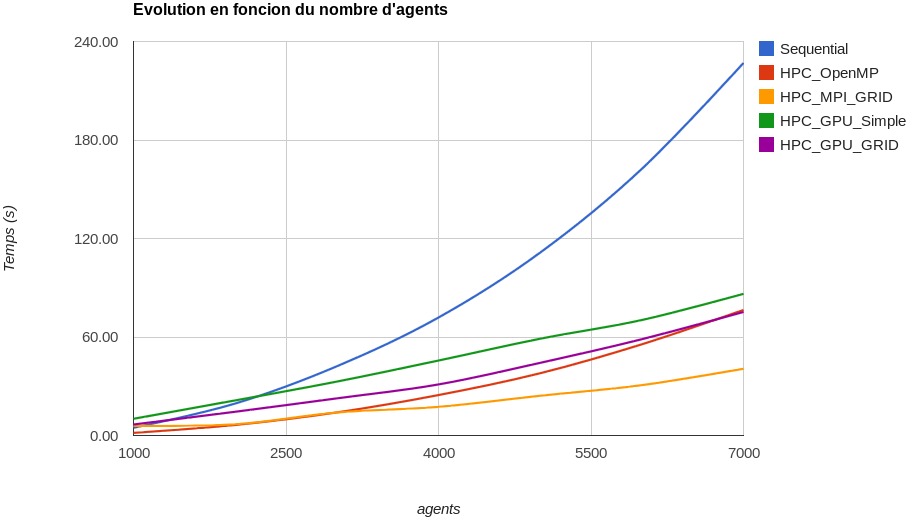
\includegraphics[width=\linewidth]{ImageGlobale}

\paragraph{Remarques}

On remarque que pour un nombre élevé d'agent, les programmes parallèle sont bien plus rapide que le programme séquentiel.

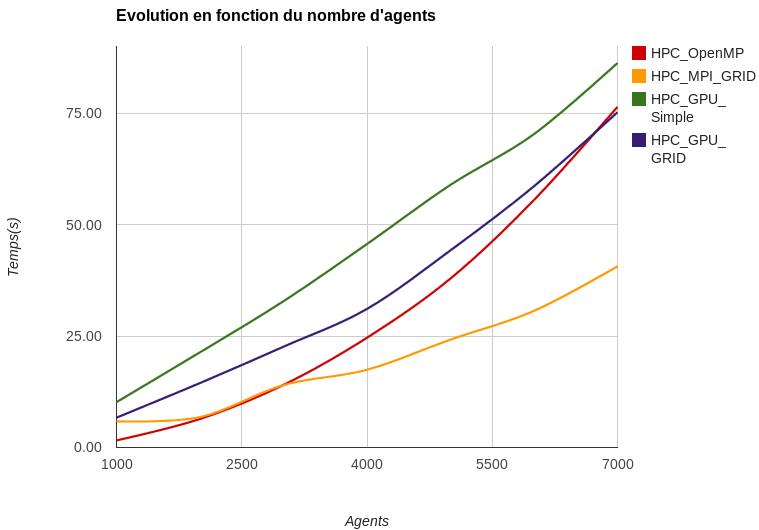
\includegraphics[width=\linewidth]{ImageGlobalLight}

\paragraph{Remarques}

Les programmes à base de grille évoluent de manière moins quadratique que les autres.

Le programme HPC\_Open\_MP bénéficie de la mémoire partagé et offre de bonne performance pour un nombre faible et moyen d'agents.
En revanche sont comportement quadratique va finir par le disqualifier.
Il se fait dépasser par HPC\_MPI\_GRID à partir de 3000 agents puis par HPC\_GPU\_GRID à partir de 7000 agents.

\subsection{Rayon d'action}

Dans ce graphique, nous nous intéressons à l'impact du rayon d'action maximum -max(rc,ra,rs)- sur les performances de la version GPU avec découpage spatial (HPC\_GPU\_Grid).
Nous affichons le temps de calcul de l'accélération, le temps utile, et le temps d'exécution total afin de connaître le surcoût engendré par la mise à jour des structures utilisées.
\paragraph{}
À titre d'information, le temps de calcul total pour HPC\_GPU\_simple est de 16.25s.
\paragraph{}
Finalement, ces tests n'ont pas étés effectués sur les machines de l'ENSIMAG, ce qui explique les temps d'exécution différents.

Nous utilisons 10000 agents.

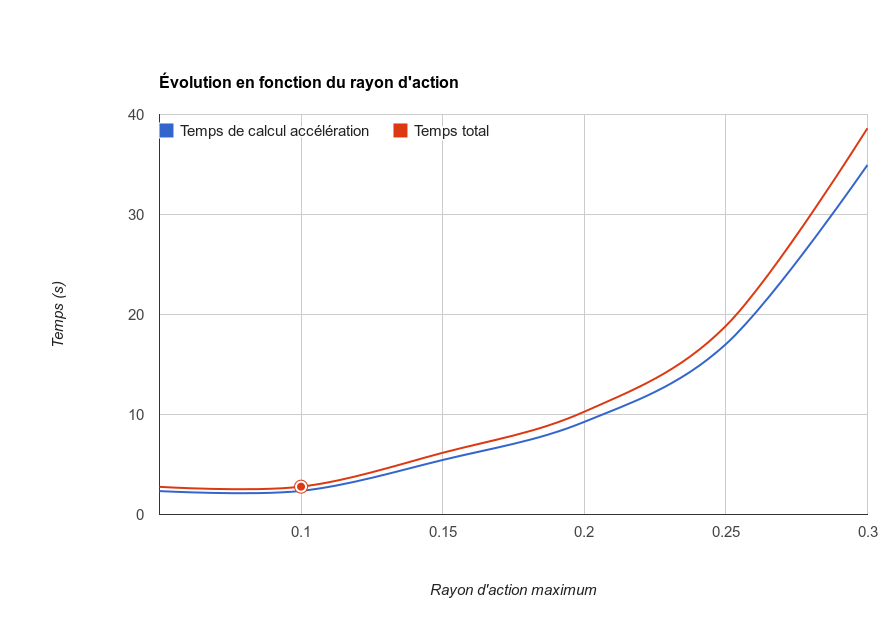
\includegraphics[width=\linewidth]{RadiusPerf}

Nous pouvons donc voir que le découpage spatial est contre-productif si $RMax > 0.23$ par contre, plus ce rayon est faible, plus l'algorithme est performant, avec une limite tout de même étant donné qu'il ne peut y avoir plus de 512 cellules dans la grille.
\paragraph{}
\begin{tabular}{|r|c|}
	\hline
	RMax & $\frac{\text{Temps utile}}{\text{Temps total}}$ \\
	\hline
	0.3 & 0.9 \\
	\hline
	0.25 & 0.9 \\
	\hline
	0.2 & 0.9 \\
	\hline
	0.15 & 0.88 \\
	\hline
	0.1 & 0.85 \\
	\hline
	0.05 & 0.84 \\
	\hline
\end{tabular}
\paragraph{}
Nous pouvons aussi constater que le ratio $\frac{\text{Temps utile}}{\text{Temps total}}$ augmente avec le rayon, ce qui est dû au fait que, plus le rayon est grand, plus il y a d'agents par cellules et moins il y a de cellules. Le calcul de l'accélération (ou plutôt de la nouvelle vitesse)  est une fonction quadratique du nombre d'agents par cellule alors que le temps de mise à jour est une fonction linéaire du même paramètre, ce qui explique cette évolution.


\section{Conclusion}

Nous avons expérimenté plusieurs façon d'implémenter la simulation des boids à travers 6 programmes différents en utilisant OpenMP et Cuda.
Nous avons estimé la complexité des ces algorithmes.
Enfin, nous avons présenté des benchmarks de ceux-ci.

\end{document}

